% This chapters elaborates some discussions in the preliminary sections, and provides useful tools that will be commonly used in subsequent proofs and analyses.

\section{The Tree Privacy Mechanism}
\label{app:prelim:tree-mechanism}

\begin{figure}[!ht]
    \centering
    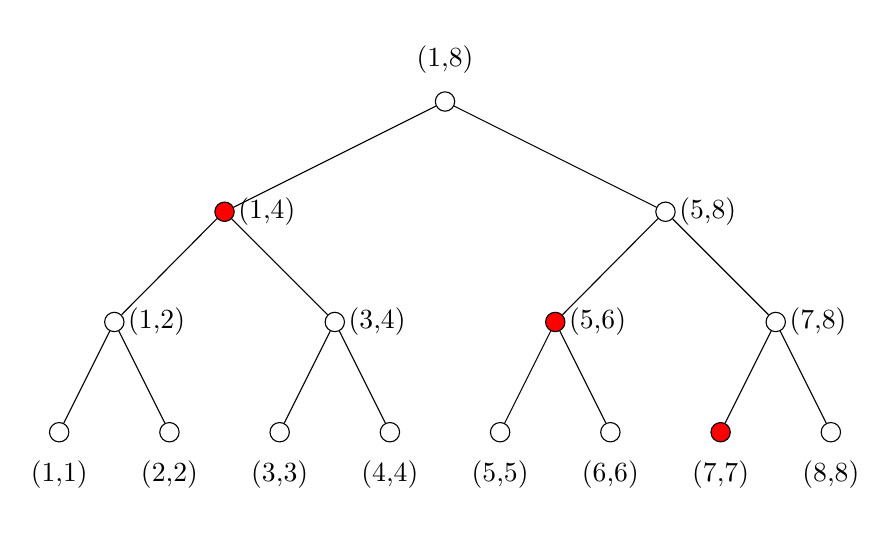
\begin{tikzpicture}[
    level 1/.style={sibling distance=56mm},
    level 2/.style={sibling distance=28mm},
    level 3/.style={sibling distance=14mm},
    level distance=14mm,
    every node/.style={
        circle,
        draw,
        minimum size=7pt,
        inner sep=0pt,
    },
    edge from parent/.style={draw, -},
    ]
    \node[label=above:{\mbox{(1,8)}}] {}
        child {
            node[label=east:{\mbox{(1,4)}},fill=red] {}
            child {
                node[label=east:{\mbox{(1,2)}}] {}
                child { node[label=below:{(1,1)}] {} }
                child { node[label=below:{(2,2)}] {} }
            }
            child {
                node[label=east:{\mbox{(3,4)}}] {}
                child { node[label=below:{(3,3)}] {} }
                child { node[label=below:{(4,4)}] {} }
            }
        }
        child {
            node[label=east:{\mbox{(5,8)}}] {}
            child {
                node[label=east:{\mbox{(5,6)}},fill=red] {}
                child { node[label=below:{(5,5)}] {} }
                child { node[label=below:{(6,6)}] {} }
            }
            child {
                node[label=east:{\mbox{(7,8)}}] {}
                child { node[label=below:{(7,7)},fill=red] {} }
                child { node[label=below:{(8,8)}] {} }
            }
        };
    \end{tikzpicture}
    \caption{An illustration of the {\tree} mechanism using a binary tree. For $n=7$, $\mathsc{Node}(7)=\{4,6,7\}$ and $\tree(7)=\vecr_4 + \vecr_6 + \vecr_7$ with a total noise of order $O(\log(n))$.}
    \label{fig:tree-illustration}
\end{figure}


We introduce several notations for analyzing the tree mechanism. Consider a complete binary tree with $n=2^m$ leaves. We index each node in the tree as follows: the leaf nodes are indexed by $(i,i)$ in an ascending order $i=1,\ldots,n$ from left to right, and every other node is indexed by $(i,j)$ where $i$ is its left-most child leaf and $j$ is its right-most child leaf (see Figure \ref{fig:tree-illustration} for illustration). 

Let $\setT$ be the set of all nodes in this tree. It's worth noting that there exists an injective mapping $\phi:[n]\mapsto \setT$ that maps $i\in[n]$ into a node by iteratively moving the leaf $(i,i)$ upwards untill it is a left child. For example, $1\mapsto (1,1) 4 \mapsto (1,4), 6\mapsto (5,6)$, etc. Under this mapping, the {\node} subroutine picks at most one node per layer, thus $|\node(n)|=O(\log(n))$.

% Let $\setT$ be the set of all nodes in this tree. We can define a total order $<$ on $\setT$ such that $(a,b) < (c,d)$ if either $b < d$ or $b=d, a<c$. In other words, we compare rightmost child first and break tie with leftmost child. We assume $(\setT,<)$ is sorted in ascending order.


\subsection{Implementation Details}
\label{app:prelim:tree-mechanism:implementation}

\begin{algorithm}[!ht]
    \begin{algorithmic}[1]
        \Statex \textbf{Input:} Natural number $n\in\NN$; distributions $\calR_1,\ldots,\calR_n$
        \State Initialize $R_0 \gets \{\}$.
        \For {$k=1,\ldots,n$}
            \State Sample $\vecr_k \sim \calR_k$ independently.
            {\color{green}
            \State Buffer $R_k \gets R_{k-1} + \{\vecr_k\}$.
            \State Update $R_k \gets R_k - \{\vecr_i: i \in \node(k-1)-\node(k)\}$.
            }
        \EndFor
        \Statex \textbf{Return:} $\tree(k;\sigma_1,\ldots,\sigma_T) = \sum_{\vecr\in R_k} \vecr$.
    \end{algorithmic}
    \caption{Practical Implementation of the {\tree} Mechanism}
    \label{alg:app:tree-practical}
\end{algorithm}

Algorithm \ref{alg:app:tree-practical} presents a practical implementation of the {\tree} mechanism that is essentially equivalent to the presentation in the main body (Algorithm \ref{alg:DP-OTB:tree}) and requires only $O(\log(n))$ memory space. The key is to sample random noises on-the-fly, and to prune unnecessary noises in the memory buffer (highlighted in green). 

To prove this implementation is equivalent to Algorithm \ref{alg:DP-OTB:tree}, it suffices to show that $\calI_k=\node(k)$ by induction, where $\calI_k\coloneqq\{i:\vecr_i\in R_k\}$ is the index set of all noises buffered in $R_k$. For $k=1$, it's trivial that $\calI_1=\{1\}$. Now suppose $\calI_{k-1}=\node(k-1)$, then the highlighted code implies
\begin{align}
    \calI_k 
    &= \calI_{k-1} + \{k\} - (\node(k-1) - \node(k)) \notag\\
    &= \node(k-1) \cap \node(k) + \{k\},
    \label{eq:app:tree-mechanism:1}
\end{align}
where the second line is from $A-(A-B)=A\cap B$ for set $A,B$.
Clearly, $\calI_k\subseteq \node(k)$ because $k\in\node(k)$. For the converse direction, the key identity is that $\node(k) = \{i=(b_m b_{m-1} \ldots b_1)_2 : i\le k, m\in\NN, b_m \ge \cdots \ge b_1, b_j\in\{0,1\}\}$ by construction. Hence, $\node(k)-\{k\} \subseteq \node(k-1)$.
Altogether, we prove that $\calI_k=\node(k)$.

Moreover, this also implies the buffer size is $|R_k| = |\node(k)| = O(\log(k))$.


\subsection{Privacy Guarantee: Proof of Theorem \ref{thm:DP-OTB:tree}}
\label{app:prelim:tree-mechanism:privacy}

Before we prove the main theorem, we first prove a more general composition of RDP mechanisms. For two datasets $\calZ_T,\calZ_T'\in\Xi^T$, we denote $\calZ_T\simeq_k \calZ_T'$ if $\calZ_T,\calZ_T'$ are neighbors and they differ at the $k$-th entry. We consider the following setup. Let $\calX_i$ be auxiliary domains which are Banach spaces. Let $\calM_1,\ldots,\calM_n$ be a sequence of randomized algorithms such that $\calM_1:\calZ_T\mapsto \vecx_1\in\calX_1$ and $\calM_i:(\vecx_1,\ldots,\vecx_{i-1},\calZ_T)\mapsto \vecx_i\in\calX_i$ iteratively. $\calM$ is the composition such that $\calM:\calZ_T\mapsto (\vecx_1,\ldots,\vecx_n)$.

Let $P_i(\vecy_1,\ldots,\vecy_{i-1},\calZ_T)$ be the output distribution of $\calM_i$. Note that $\vecy_j$'s are arbitrary auxiliary inputs and are not necessarily previous outputs. In this chapter, we reserve $\vecx_i$ for the output of $\calM_i$ to avoid confusion. For $t\in[T]$, define
\begin{align*}
    \IN(t) &\coloneqq \{ i\in[n] : P_i(\ldots,\calZ_T) = P_i(\ldots,\calZ_T'), \, \forall \vecy_j\in\calX_j, \forall \calZ_T\simeq_t \calZ_T' \}, \\
    \OUT(t) &\coloneqq [n]-\IN(t).
\end{align*} 
In other words, $\IN(t)$ denotes the index set of sub-algorithms that are \emph{independent} of the $k$-th entry. Under this setup, we have the following privacy guarantee, which states that the privacy budget of the composition is bounded by the total privacy budget of all sub-algorithms that are \emph{dependent} on a single data.

\begin{lemma}[Advanced Composition]
\label{lem:app:tree-mechanism:RDP-composition}
If $\calM_i(\vecx_1,\ldots,\vecx_{i-1},\cdot)$ is $(\alpha,\rho_i)$-RDP for any auxiliary inputs, then $\calM$ is $(\alpha, \rho)$-RDP, where
\begin{equation}
    \rho \le \max_{t\in[T]} \sum_{i\in \OUT(t)} \rho_i.
    \label{eq:app:tree-mechanism:advanced-composition}
\end{equation}
\end{lemma}

\begin{proof}
Suppose $\calZ_T\simeq_t \calZ_T'$ for an arbitrary $t$. With a slight abuse of notation, let $P_i(\vecx_i|\vecx_1,\ldots,\vecx_{i-1})$ be the output distribution of $\calM_i$ given the previous outputs and dataset $\calZ_T$. Then $P=P_1\times\dotsm\times P_n$ is the output distribution of $\calM(\calZ_T)$. We define $Q_i$ and $Q$ similarly with respect to $\calZ_T'$.

For each $i\in[n]$, if $i\in\IN(t)$, then $P_i=Q_i$; if $i\in\OUT(t)$, since $\calM_i$ is $(\alpha,\rho_i)$-RDP, $D_\alpha(P_i\|Q_i)\le \rho_i$. Therefore, upon applying additivity of R\'enyi divergence \citep[Theorem 28]{mironov2017renyi},
\begin{equation*}
    D_\alpha(P \| Q) = \sum_{i=1}^n D_\alpha(P_i\|Q_i) \le \sum_{i\in\OUT(t)} \rho_i.
    \qedhere
\end{equation*}
\end{proof}

Now we are ready to prove the main theorem (Theorem \ref{thm:DP-OTB:tree}).

% \TreeMechanism*

\begin{proof}
The proof sketch is to reduce the streaming sum composition into the advanced composition setup in Lemma \ref{lem:app:tree-mechanism:RDP-composition}.
Let $\setT$ be set of all nodes of the binary tree with $n=2^m$ leaf nodes, and $\phi:[n]\mapsto \setT$ be the aforementioned injective mapping. We can rewrite each streaming sum $\calS_k$ as follows:
\begin{align*}
    \calS_k(\vecx_{i:k-1},\calZ_T) = \sum_{i=1}^k \vecx_i = \sum_{\substack{i\in\node(k),\\(a,i)=\phi(i)}} \sum_{j=a}^i \vecx_j.
\end{align*}
Consequently, for each $i\in[n]$ and $\phi(i)=(a,i)$, by defining 
\begin{align*}
    \calA_i:(\vecx_1,\ldots,\vecx_{i-1},\calZ_T) \mapsto \sum_{j=a}^i \calM_j(\vecx_{1:j-1},\calZ_{p_j}),
\end{align*}
we establish that 
\begin{align*}
    \calS_k(\vecx_{i:k-1},\calZ_T) = \sum_{i\in\node(k)} \calA_i(\vecx_1,\ldots,\vecx_{i-1},\calZ_T).
\end{align*}
Clearly, the composition $(\calS_1,\ldots,\calS_n)$ is a post-processing of $(\calA_1,\ldots,\calA_n)$. Therefore, the problem reduces to making the composition $(\calA_1,\ldots,\calA_n)$ RDP via Lemma \ref{lem:app:tree-mechanism:RDP-composition}.

Let $\tilde\calA_i = \calA_i + \vecr_i$, where $\vecr_i\sim \sigma_i\calR$ independently, $\calR$ be an $(\alpha,\RDPdist)$-RDP distribution, and $\phi(i)=(a,i)$. Note that $\calM_j$'s use independent data $\calZ_{p_j}$, so the sensitivity of $\calA_i$ is bounded by $\max_{j\in [a,i]} s_j$, where $s_j=\sens(\calM_j)$. Consequently, $\tilde\calA_i$ is $(\alpha,\alpha\rho_i^2/2)$-RDP, where $\rho_i = \RDPdist\cdot \max_{j\in [a,i]}s_j / \sigma_i$ (by Theorem \ref{thm:DP-OTB:RDP-mechanism}). Also note that 
\begin{align*}
    \tilde\calS_k 
    &= \sum_{i\in\node(k)} \left(\calA_i + \vecr_i\right) 
    = \calS_k + \tree(k).
\end{align*}
Hence, by Lemma \ref{lem:app:tree-mechanism:RDP-composition}, $\tilde\calS$ is $(\alpha,\alpha\rho^2/2)$-RDP where
\begin{align*}
    \alpha\rho^2/2 
    &\le \max_{t\in[T]}\sum_{i\in \OUT(t)} \alpha\rho_i^2/2 \\
    &\le \max_{t\in[T]}\sum_{i\in \OUT(t)} \alpha \left(\frac{\RDPdist\cdot \max_{j\in [a,i]}s_j}{\sigma_i}\right)^2 /2, \\
    \iff \rho 
    &\le \RDPdist \cdot \max_{t\in[T]} \sqrt{|\OUT(t)|} \max_{i\in\OUT(t)} \frac{\max_{j\in [a,i]}s_j}{\sigma_i}.
\end{align*}
Note that $\calA_i$ depends on data $\xi_t$ if and only if $\xi_t\in\calZ_{p_j}$ where $(j,j)$ is a leaf node of the node $\phi(i)$. Hence, $|\OUT(t)|\le \log_2(2n)$. This concludes the proof.
\end{proof}